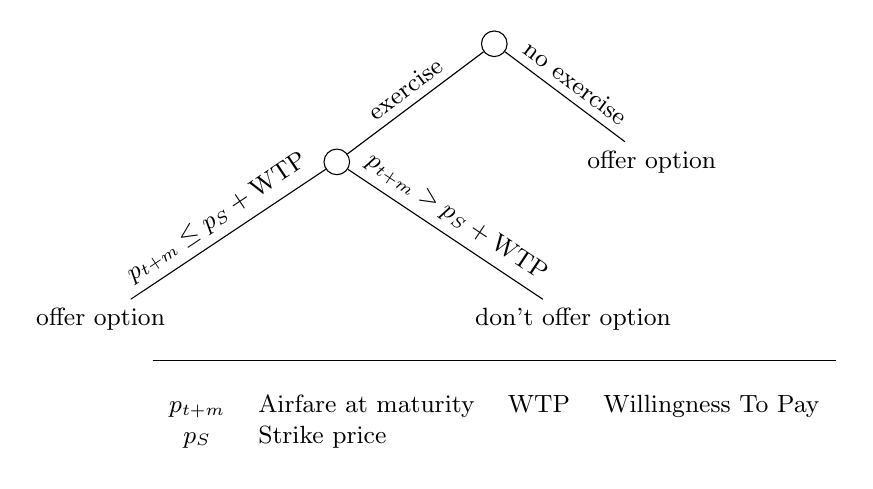
\begin{tikzpicture}[grow=down, sloped,
                    level 1/.style={sibling distance=4cm, level distance=1.5cm}, level 2/.style={sibling distance=6cm, level distance=2cm},
                    bag/.style={circle, draw, minimum width=1em}]
\small
\node[bag] {}
    child {
        node[bag] {}
        child {
                node[align=center] {offer option}
                edge from parent
                node[above] {$p_{t+m} \le p_S + \mbox{WTP}$}
            }
            child {
                node[align=center] {don't offer option}
                edge from parent
                node[above] {$p_{t+m} > p_S + \mbox{WTP}$}
            }
        edge from parent
        node[above] {exercise}
    }
    child {
        node {offer option}
        edge from parent
        node[above] {no exercise}
    };

\node at (0,-4.6)
{
\begin{tabular}{clcl}
\hline \\
$p_{t+m}$ & Airfare at maturity  &  $\mbox{WTP}$  & Willingness To Pay\\
$p_S$ & Strike price
\end{tabular}
};
\end{tikzpicture}
